\chapter{Determinação do som gerado por desprendimento de vórtices}

\section{Questão 1 - O espectro do histórico de pressão medido a 90 o em NPS.}

\begin{figure}[h!]
    \centering
    \hspace{-1.cm}
    \includegraphics[width=0.8\textwidth]{Mach_0.1/fft_pressure.eps}
    \caption{Gráfico do espectro de frequências do histórico de pressão em Mach 0.1.}
\end{figure}

\begin{figure}[h!]
    \centering
    \hspace{-1.cm}
    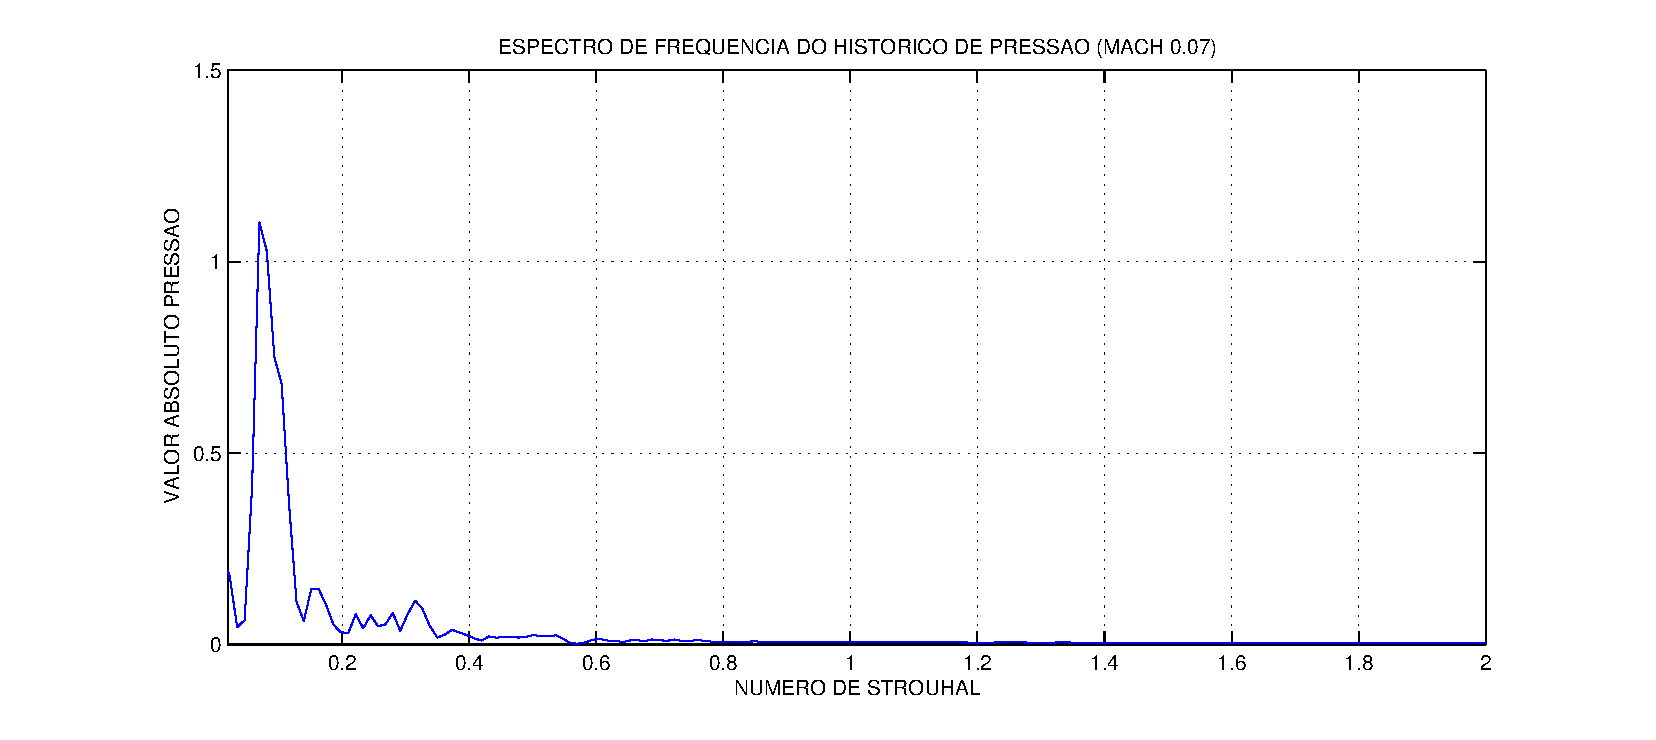
\includegraphics[width=0.8\textwidth]{Mach_0.07/fft_pressao.eps}
    \caption{Gráfico do espectro de frequências do histórico de pressão em Mach 0.07.}
\end{figure}

\newpage
Para o escoamento de Mach 0.03 não um espectro de frequências significativo, pois o escoamento para número esse número Mach se comportou como estável. A estabilidade pode ser percebida no gráfico abaixo pelos níveis de amplitude da onda de pressão.

\begin{figure}[h!]
    \centering
    \hspace{-1.cm}
    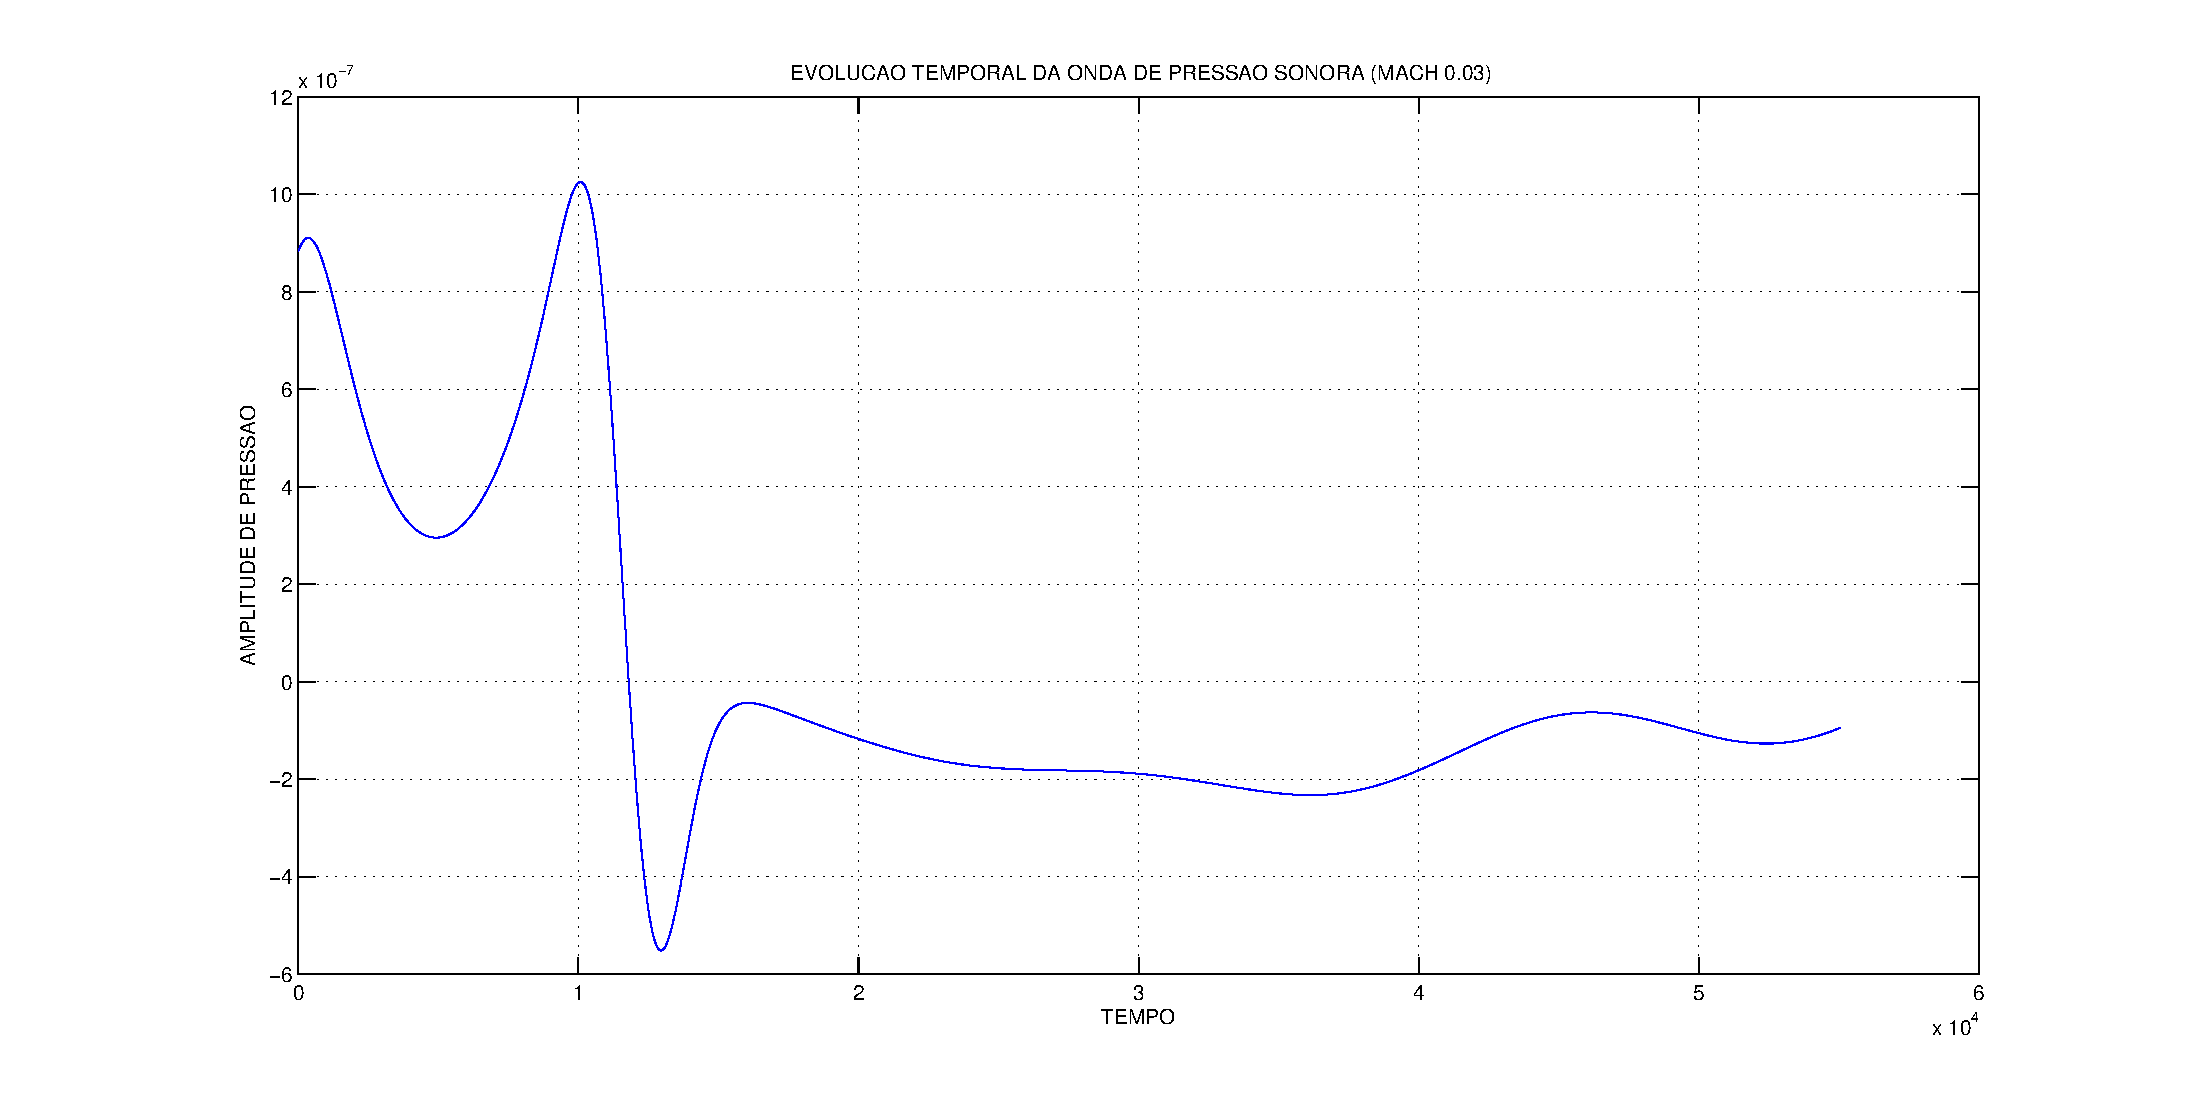
\includegraphics[width=1.\textwidth]{Mach_0.03/pressao_estabilizada_no_tempo.eps}
    \caption{Gráfico da evolução da onda sonora em Mach 0.03.}
\end{figure} 

\section{Questão 2 - Qual a frequência de pico para cada uma das velocidades? Justifique este resultado.}

As frequências de pico estão relacionadas ao número de Strouhal e pode ser encontrada pela fórmula \ref{eqn1}. Tal que $M$ é o número de Mach, $c_{o}$ é a velocidade de lattice, $st$ é o número de strouhal e $D$ é a dimensão característica.
\begin{equation}
    f = \frac{M.c_{o}.st}{D}
    \label{eqn1}
\end{equation}

Para os seguintes Mach foram encontradas as seguintes frequências de pico:
\begin{itemize}
    \item Mach 0.07: 1.428941916244324e-04 frequência de lattice;
    \item Mach 0.1: 1.178371899416027e-04 frequência de lattice.
\end{itemize}

\section{Questão 3 - Tomando-se como referência as frequências de pico para cada velocidade, plote em uma mesma figura as direcionalidades de 0 graus a 180 graus para cada número de Mach avaliado.}

\begin{figure}[h!]
    \centering
    \hspace{-1.cm}
    \includegraphics[width=0.8\textwidth]{Mach_0.1/diretividade.eps}
    \caption{Diretividade com Mach 0.1.}
\end{figure}

\begin{figure}[h!]
    \centering
    \hspace{-1.cm}
    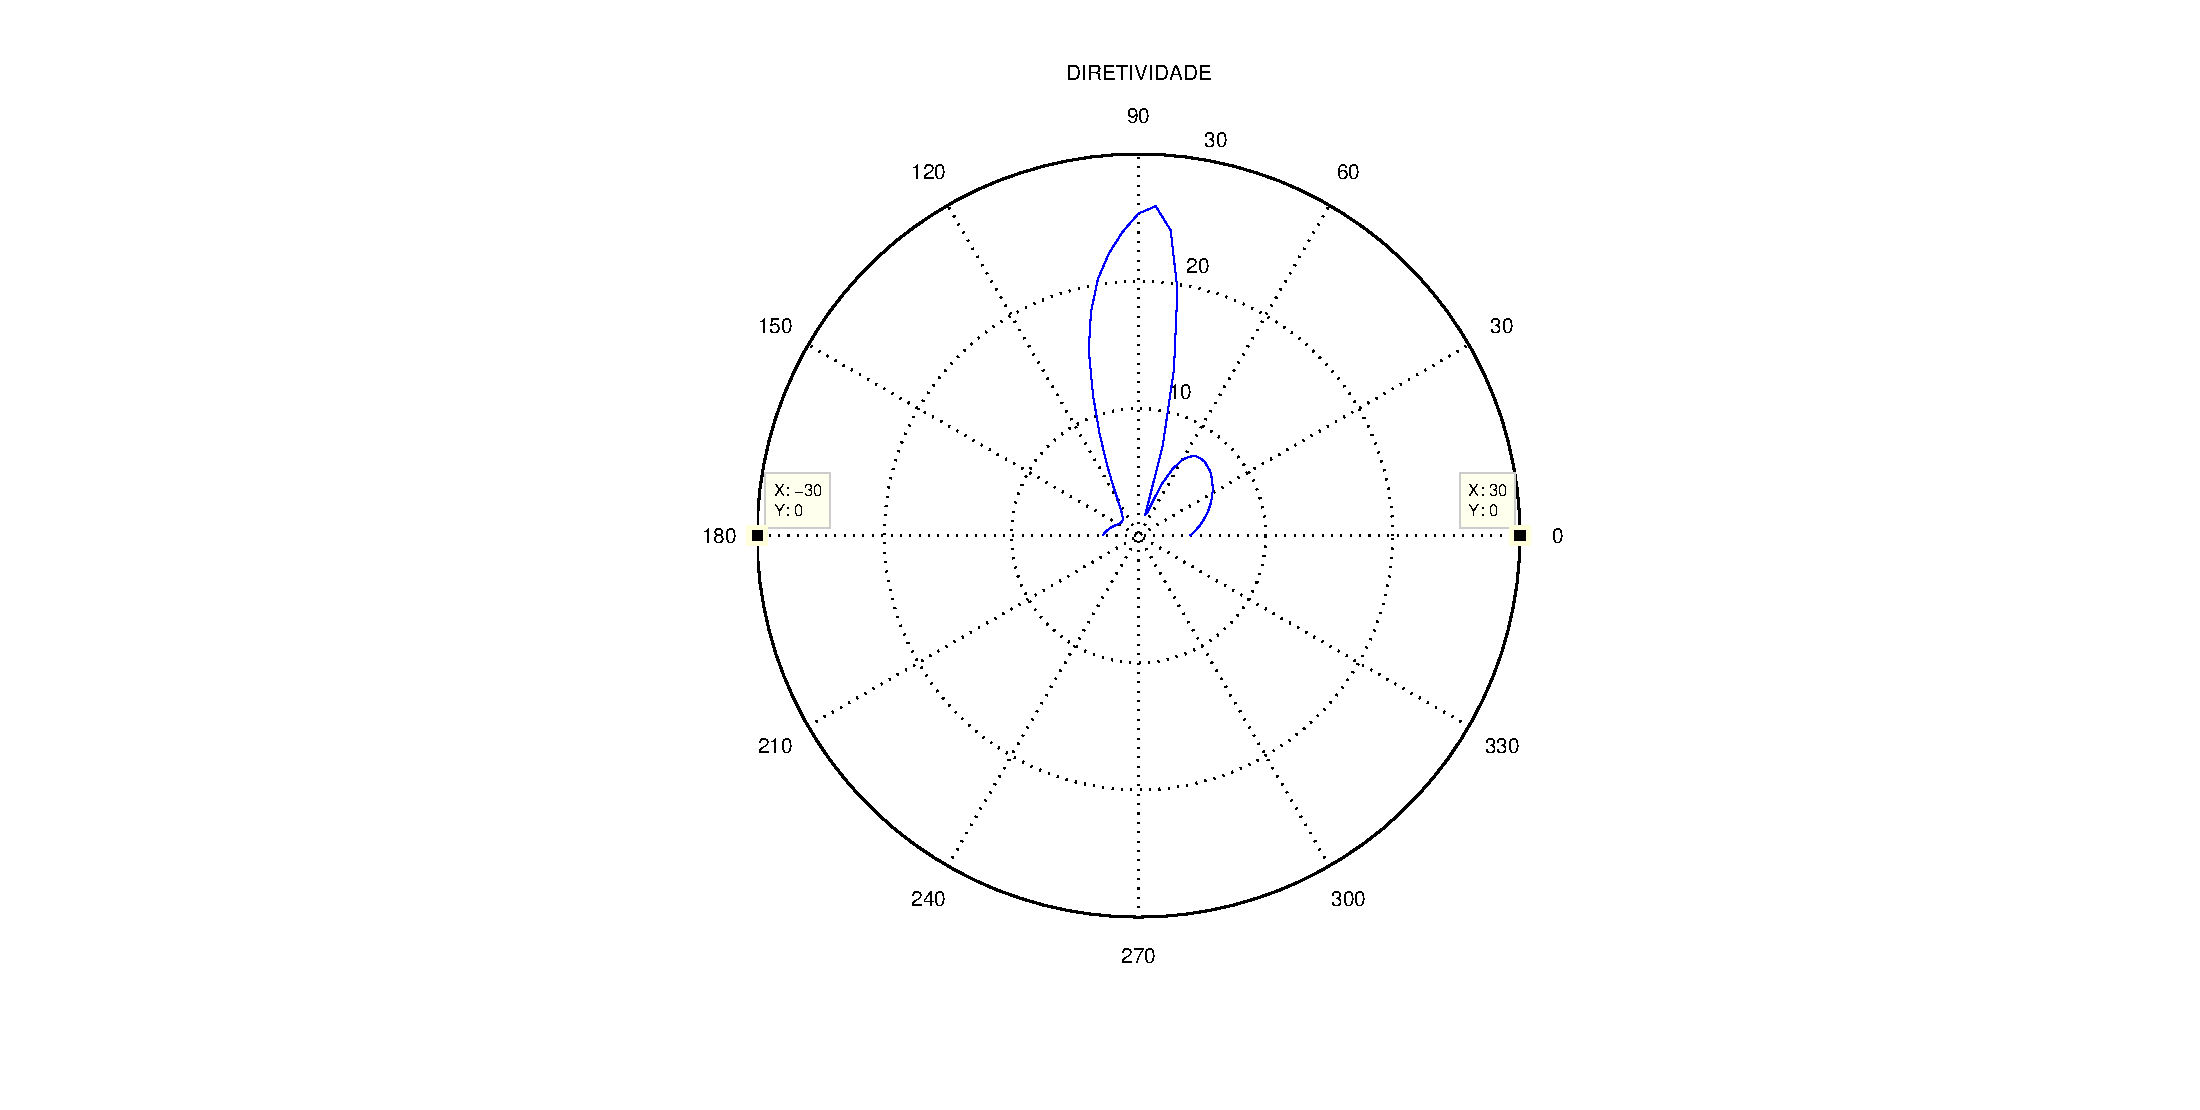
\includegraphics[width=1.1\textwidth]{Mach_0.1/diretividade_polar.eps}
    \caption{Diretividade em gráfico polar com Mach 0.1.}
\end{figure}

\begin{figure}[h!]
    \centering
    \hspace{-1.cm}
    \includegraphics[width=1\textwidth]{Mach_0.07/diretividade.eps}
    \caption{Diretividade com Mach 0.07.}
\end{figure}

\begin{figure}[h!]
    \centering
    \hspace{-1.cm}
    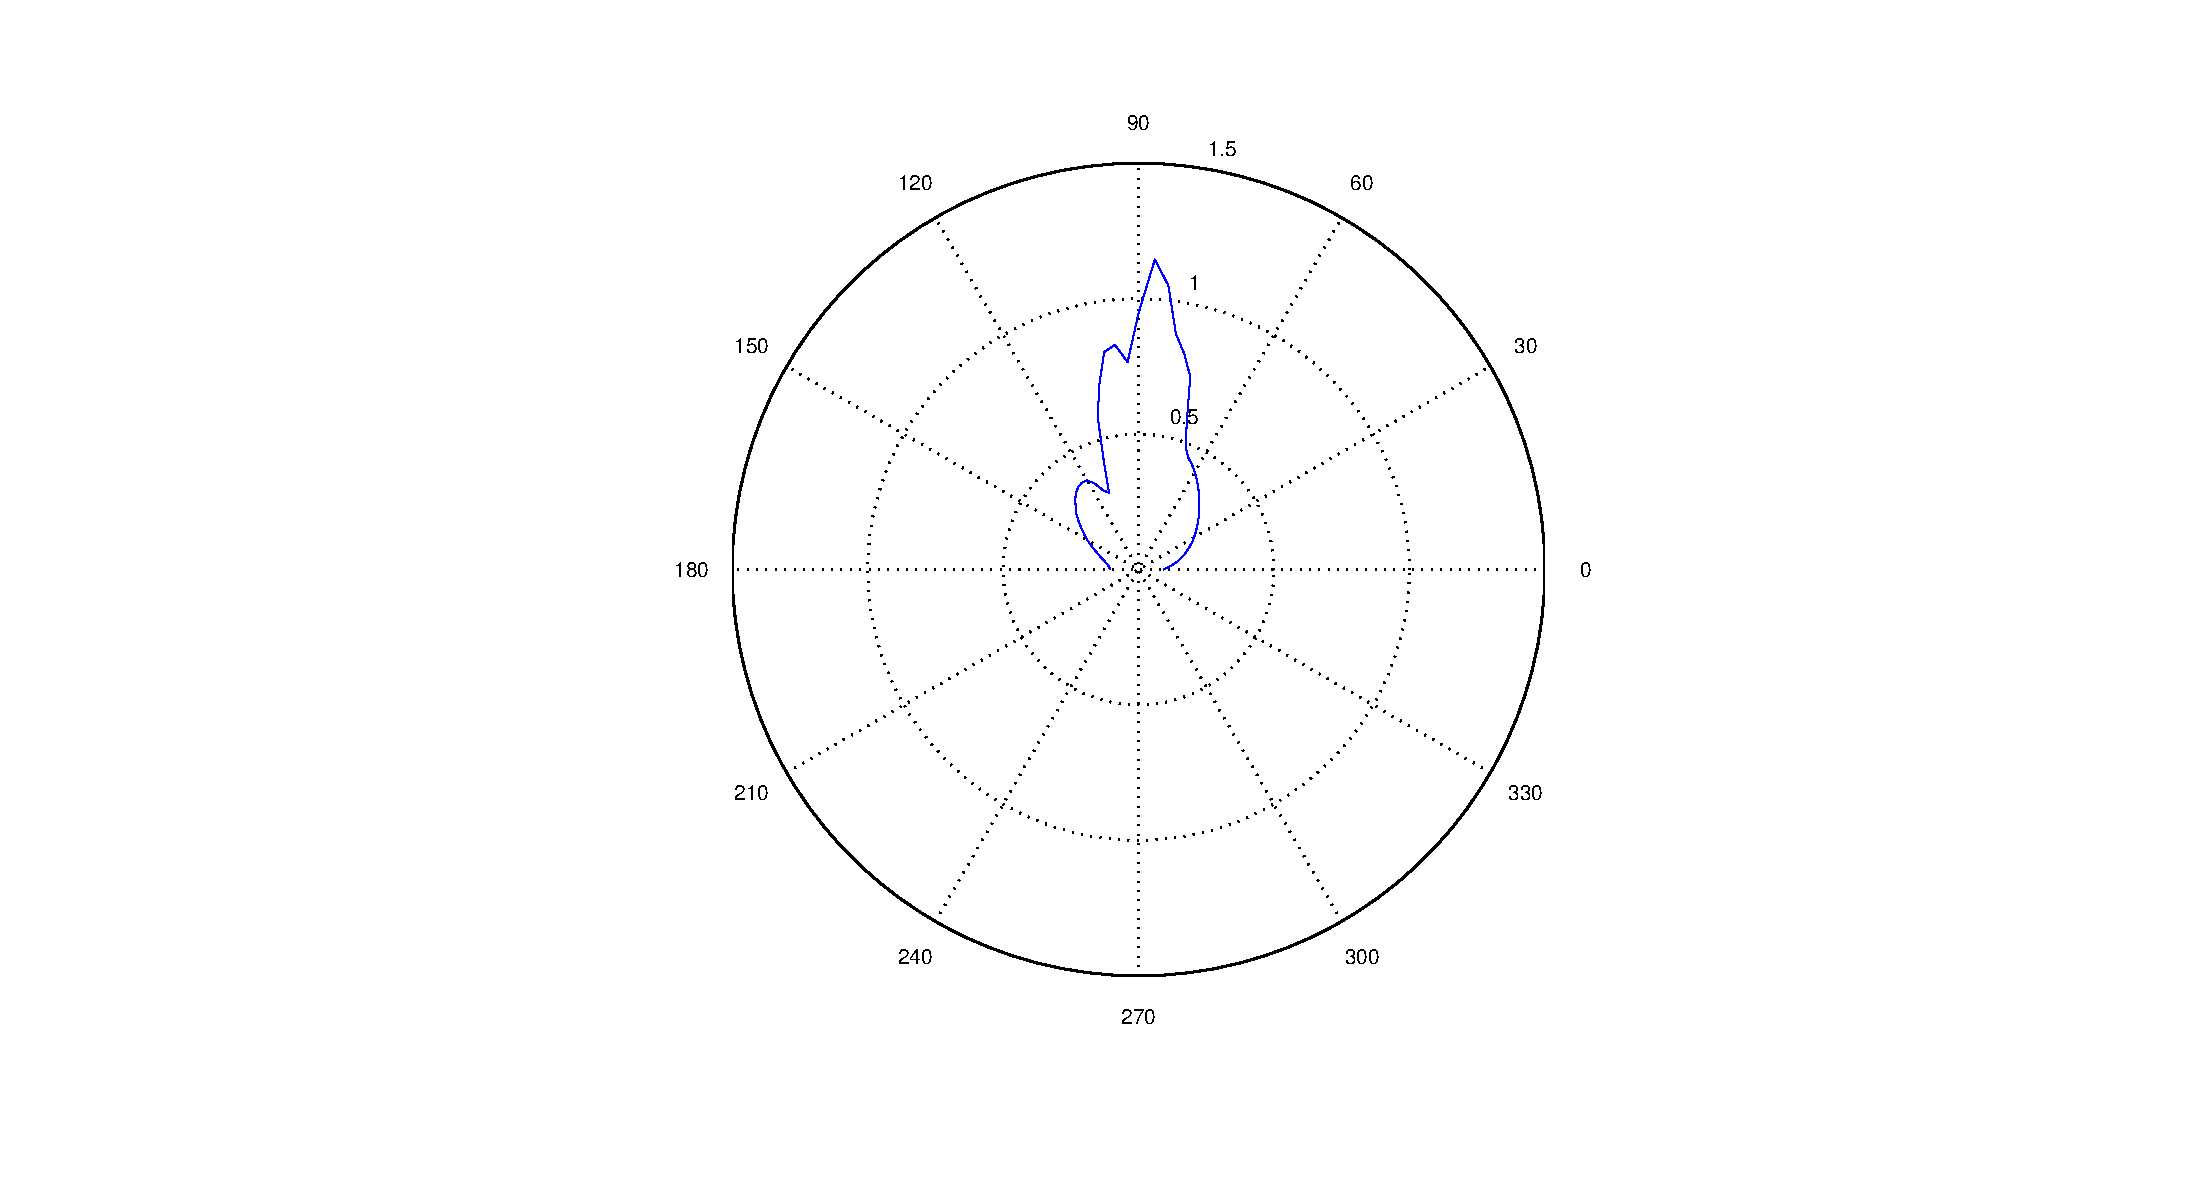
\includegraphics[width=1\textwidth]{Mach_0.07/diretividade_polar.eps}
    \caption{Diretividade em gráfico polar com Mach 0.07.}
\end{figure}

\newpage
\section{Questão 4 - Disponibiliza o gráfico do campo acústico para cada velocidade.}
\newpage
\begin{figure}[h!]
    \centering
    \hspace{-3.cm}
    \includegraphics[width=1.2\textwidth]{Mach_0.1/campo_pressao.eps}
    \caption{Campo acústico com Mach 0.1.}
\end{figure}

\begin{figure}[h!]
    \centering
    \hspace{-3.cm}
    \includegraphics[width=1.2\textwidth]{Mach_0.07/campo_pressao.eps}
    \caption{Campo acústico com Mach 0.07.}
\end{figure}

\newpage
\section{Questão 5 - Tente disponibilizar o mesmo campo acústico isolado para a frequência de pico.}
\begin{figure}[h!]
    \centering
    \hspace{-3.cm}
    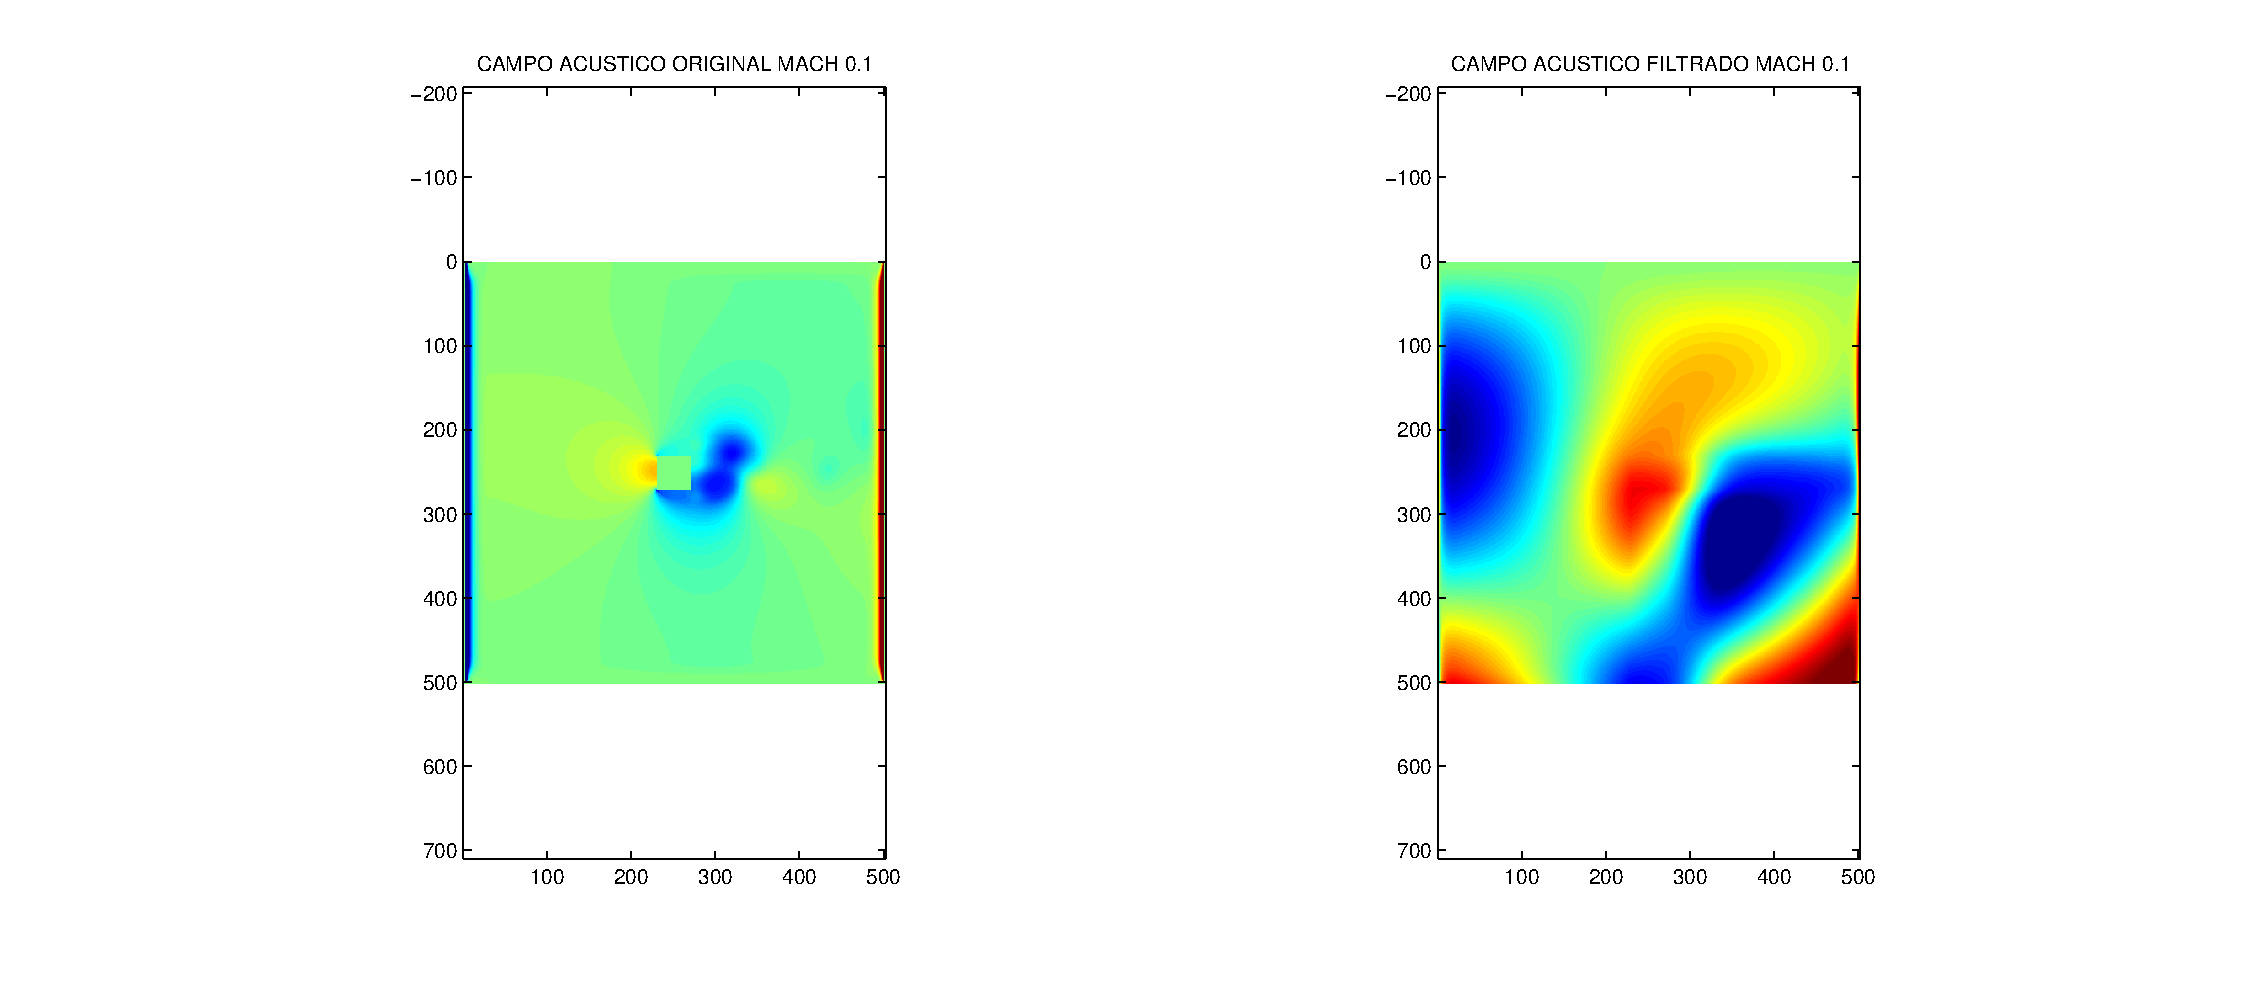
\includegraphics[width=1.2\textwidth]{Mach_0.1/campo_acustico_filtrado.eps}
    \caption{Campo acústico filtrado com Mach 0.1.}
\end{figure}

\begin{figure}[h!]
    \centering
    \hspace{-3.cm}
    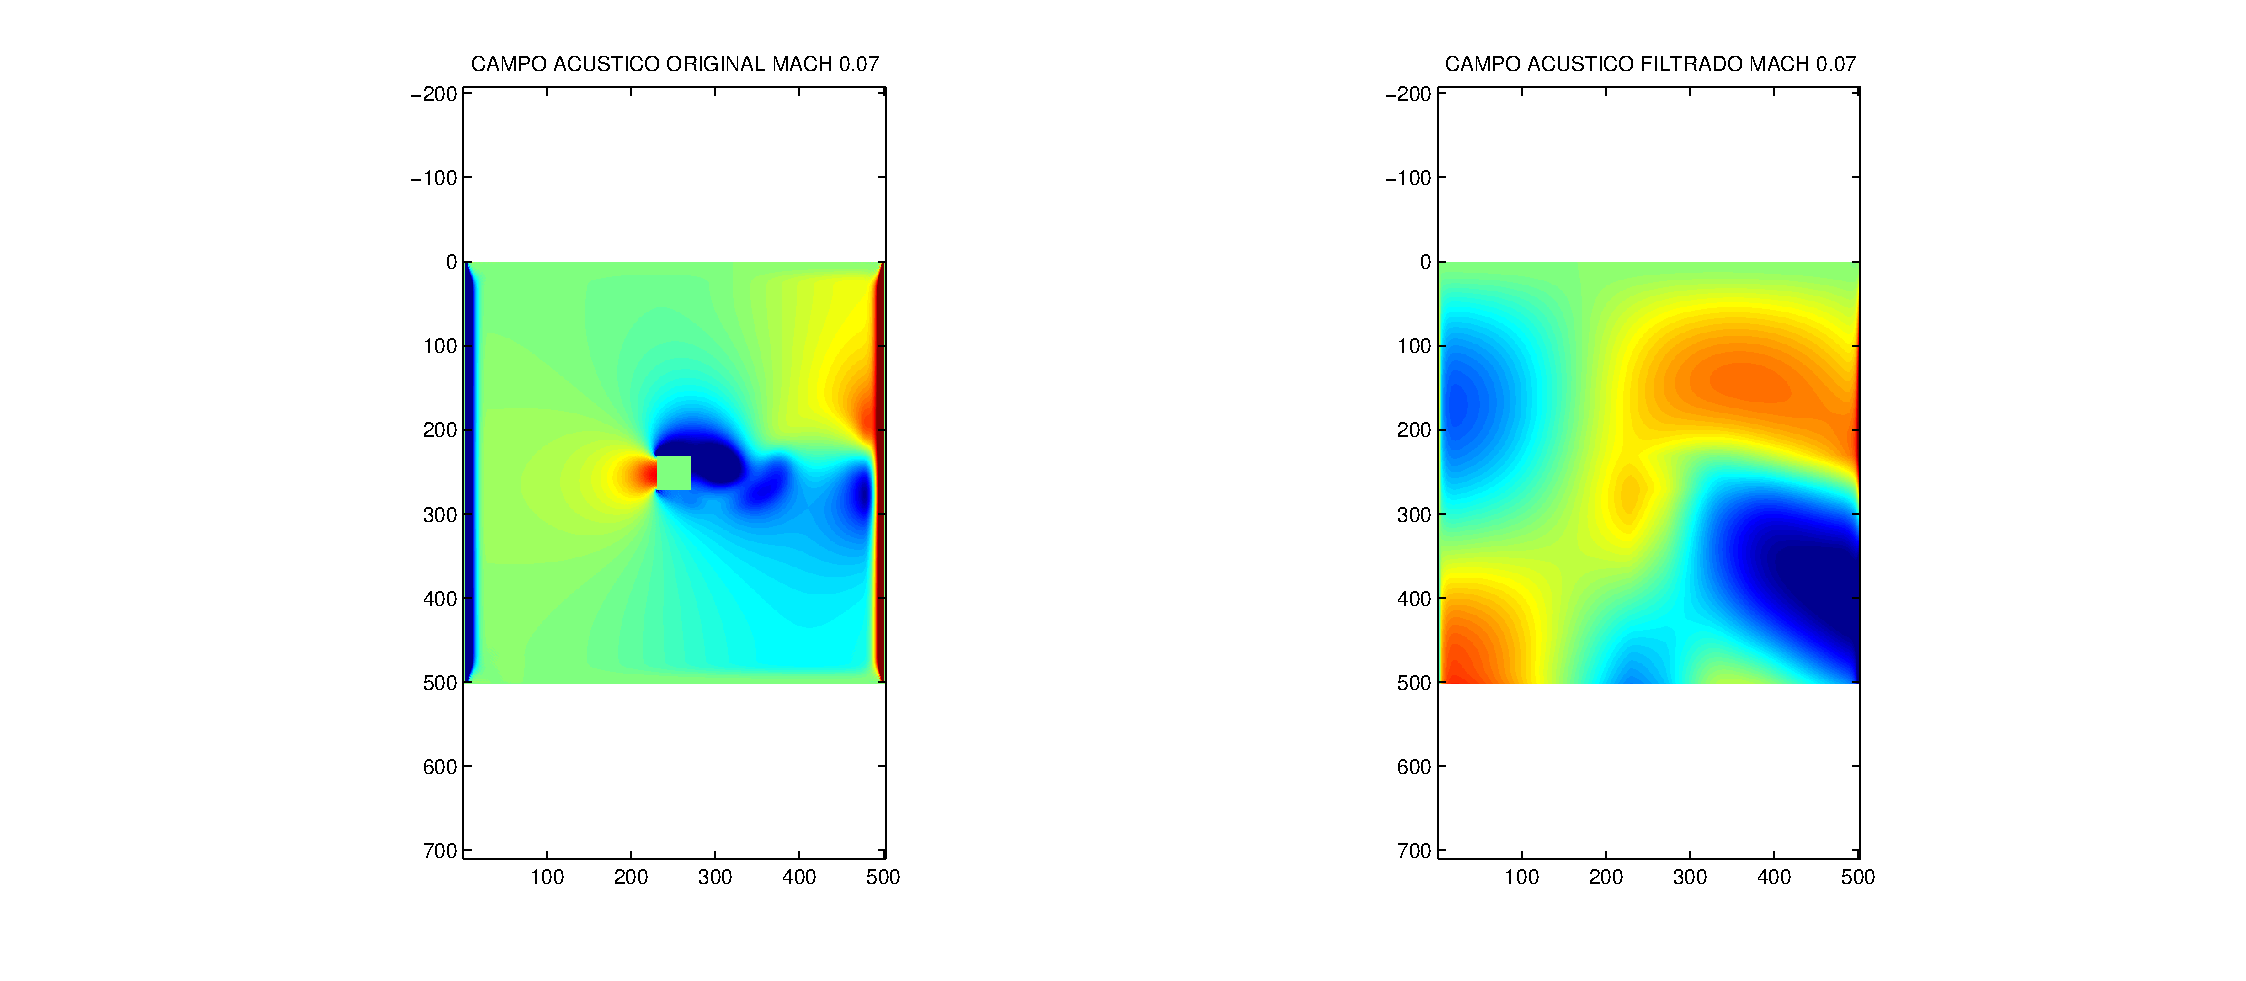
\includegraphics[width=1.2\textwidth]{Mach_0.07/campo_pressao_filtrado.eps}
    \caption{Campo acústico filtrado com Mach 0.07.}
\end{figure}

\section{Questão 6 - A partir da análise das ilustrações do ítem anterior, discuta qual o tipo de fonte que predomina no sistema modelado.}

Diante da filtragem obtida a partir da frequência de pico mais prepoderante no espectro de frequência temporal, obteve-se um campo acústico que se irradia mais aproximadamente como um dipolo, fato esse que possui aderência a teoria vigente de uma força atuando no flúido. Porém há algumas limitações a serem consideradas, a primeira é que o escoamento foi pouco desenvolvido mesmo com um número de iterações na ordem de 4.8e5, isso equivale em unidades físicas a aproximadamente 0.14 segundos, e a segunda limitação é que o comprimento de onda da frequência irradiadora filtrada é maior que as dimensões da malha lattice, isso significa que não dá para ver tão evidente a irradiação de um dipolo.


\section{Questão 7 - Para que se tenha a viscosidade cinemática do ar em condições normais de temperatura e pressão, qual deve ser o ∆x? Nesse caso, quais as dimensões físicas do anteparo?}

Para o cálculo da discretização espacial foi utilizado a seguinte fórmula:
\begin{equation}
    \Delta{x} = \frac{\nu.\sqrt{3}}{c_0.(\tau - 1/2)}
\end{equation}
Tal que $\Delta{x}$ é a discretização espacial, $\nu$ é a viscosidade física do ar, $c_0$ é velocidade física do som e $\tau$ é o período de relaxação de lattice. Segue resultado do cálculo:
\begin{figure}[h!]
    \centering
    \hspace{-1.cm}
    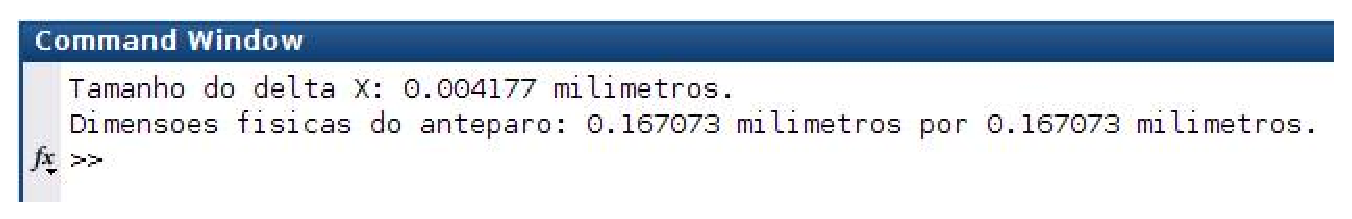
\includegraphics[width=1\textwidth]{resultado_calculo.eps}
\end{figure}




